% BEGIN B024-ADMIN
\scanpage{24}
% Independent reader B; literal shapes below are manual approximations, without rendered or metric validation.
% Vertical bars inside unsure arguments separate editorial alternatives; they are not manuscript punctuation.
% END B024-ADMIN

% BEGIN B024-P01
\unsure{Considérons|Considerons} la partition $\Pi_I^{\unsure{\circ|0}}$ de $X\setminus\bigcup_{\unsure{\alpha'|i}\in I}E_{\alpha'}$, soit $S$ l'ens des classes, notées $U_s$ $(s\in S)$. \deleted{\unsure{On a|On}} Considérons la
% END B024-P01

% BEGIN B024-G01
\figure{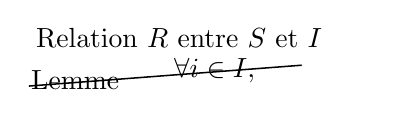
\begin{tikzpicture}[x=1ex,y=1ex,baseline=(oldlemma.base)]
\path[use as bounding box] (-.3,-1.1) rectangle (29,5.2);
\node[anchor=base west,inner sep=0,outer sep=0] (oldlemma) at (0,0) {\rlap{\uline{Lemme}}\phantom{\deleted{\uline{Lemme}}}};
\node[anchor=base west,inner sep=0,outer sep=0] (oldforall) at (12,1) {\rlap{$\forall i\in I,$}\phantom{\deleted{$\forall i\in I,$}}};
\node[anchor=base west,inner sep=0,outer sep=0] (newrelation) at (.4,3.5) {\inserted{Relation $R$ entre $S$ et $I$}};
\draw[line width=.55pt] (-.2,.3) -- (22.7,2.05);
\end{tikzpicture}}
% END B024-G01

% BEGIN B024-DISPLAY
\[
% BEGIN B024-G02
% The high point has unresolved role, hand and attachment; it is present once above the deleted glyph.
\overset{\hspace{-1ex}\unsure{\cdot}}{\deleted{\unsure{U|E}}}
% END B024-G02
(s,i)\in R\ 
% BEGIN B024-G03
\mathrel{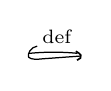
\begin{tikzpicture}[x=1ex,y=1ex,baseline=-.25ex]
\path[use as bounding box] (0,-.45) rectangle (4.6,2.5);
\node[anchor=base,inner sep=0,outer sep=0] (deflabel) at (2.45,1.2) {\scriptsize def};
\draw[line width=.45pt] (.8,.95) .. controls (.25,.88) and (-.05,.28) .. (.08,.02) .. controls (.3,-.2) and (.8,-.16) .. (1.3,-.11) -- (4.45,.12);
\draw[line width=.45pt] (.09,.34) .. controls (1.7,.5) and (3.1,.45) .. (4.18,.35);
\draw[line width=.6pt] (4.04,.52) .. controls (4.5,.28) and (4.57,.1) .. (4.43,-.05) -- (4.14,-.23);
\end{tikzpicture}}
% END B024-G03
\ \overline{U_s}\cap E_i\ne\varnothing.
\]
% END B024-DISPLAY

% BEGIN B024-P02
\uline{Lemme} Cette relation fait de
% BEGIN B024-G04
% Complete states: (S,I)\deleted{R}) | (S,I\deleted{)},R).
% The qualifier belongs to the whole right-hand correction, not to the already clear S,I letters alone.
\unsure{
\begin{tikzpicture}[x=1ex,y=1ex,baseline=(tupleprefix.base)]
\path[use as bounding box] (0,-1.1) rectangle (8.9,2.7);
\node[anchor=base west,inner sep=0,outer sep=0] (tupleprefix) at (0,0) {$(S,I$};
\node[anchor=base west,inner sep=0,outer sep=0] at (0,0) {\phantom{$(S,I)\deleted{R})$}};
\draw[line width=.6pt] (4.35,2.3) .. controls (4.55,1.2) and (4.3,.2) .. (3.9,-.55);
\draw[line width=.5pt] (5.25,1.95) -- (5.05,-.1) .. controls (5,-.2) and (4.95,-.3) .. (4.8,-.2);
\draw[line width=.5pt] (5.18,1.65) .. controls (5.9,2.35) and (6.4,2.0) .. (5.8,1.1) .. controls (5.35,.7) and (5.25,.45) .. (5.55,.2) -- (6.0,-.2);
\draw[line width=.55pt] (4.95,1.95) -- (6.65,2.5);
\draw[line width=.55pt] (4.8,1.0) -- (6.28,1.72);
\draw[line width=.55pt] (5.25,.52) -- (7.1,1.4) -- (5.7,.62);
\draw[line width=.55pt] (5.63,.2) .. controls (6.7,.2) and (8.45,.45) .. (8.0,-.1) .. controls (7.6,-.5) and (7.15,-.67) .. (7.42,-.95) .. controls (7.9,-1.1) and (8.55,-.1) .. (8.65,1.05) .. controls (8.7,1.6) and (8.55,2.1) .. (8.45,2.25);
\end{tikzpicture}}
% END B024-G04
% END B024-P02

% BEGIN B024-P03
\noindent
% BEGIN B024-G05
\llap{\begin{tikzpicture}[x=.18pt,y=-.18pt,baseline=(ruletop)]
\path[use as bounding box] (-10,0) rectangle (45,405);
\coordinate (ruletop) at (25,0);
\draw[line width=.45pt] (13,39) .. controls (18,28) and (18,11) .. (20,4) .. controls (23,-1) and (25,3) .. (25,15) .. controls (22,81) and (20,117) .. (23,163) .. controls (30,241) and (27,324) .. (29,396);
\node[anchor=base west,inner sep=0,outer sep=0] at (0,0) {\unsure{\begin{tikzpicture}[x=.18pt,y=-.18pt,baseline=0pt]
\path[use as bounding box] (-10,0) rectangle (45,405);
\draw[black!65,line width=.25pt] (1,82) -- (-2,91) -- (-5,98);
\draw[black!55,line width=.3pt] (-7,103) -- (-8,107);
\end{tikzpicture}}};
\end{tikzpicture}\quad}
% END B024-G05
un graphe strict ayant $S$ comme \unsure{ens des|ens de}
% BEGIN B024-G06
\begin{tikzpicture}[x=1ex,y=1ex,baseline=(sommets.base)]
\node[anchor=base west,inner sep=0,outer sep=0] (sommets) at (0,0) {sommets};
\node[anchor=base west,inner sep=0,outer sep=0] at (0,0) {\unsure{\begin{tikzpicture}[x=1ex,y=1ex,baseline=0pt]
\path[use as bounding box] (0,0) rectangle (7,2.5);
\fill (5.05,1.8) -- (5.2,2.04) -- (5.32,1.97) -- (5.2,1.76) -- cycle;
\end{tikzpicture}}};
\end{tikzpicture}
% END B024-G06
, $I$ comme ens. \unsure{de |d'}\unsure{arêtes|arètes|aretes}.). \deleted{Cette relation}
% BEGIN B024-G07
% Complete word candidates: Le | Ce. The detached upper hooked run stays with the qualified word.
\unsure{
\begin{tikzpicture}[x=.2pt,y=-.2pt,baseline=(lebase)]
\path[use as bounding box] (0,0) rectangle (85,65);
\coordinate (lebase) at (0,57);
\node[anchor=base west,inner sep=0,outer sep=0] at (0,57) {\phantom{Le}};
\draw[line width=.6pt] (2,14) -- (7,55) .. controls (17,56) and (26,53) .. (31,57) .. controls (39,63) and (46,53) .. (53,49) .. controls (48,55) and (49,57) .. (58,56) -- (83,55);
\fill (14,15) -- (14,8) -- (25,0) -- (32,1) -- (36,0) -- (37,4) -- (33,6) -- (27,5) -- (18,13) -- cycle;
\end{tikzpicture}}
% END B024-G07
graphe est un \uline{arbre}
% END B024-P03

% BEGIN B024-P04
\unsure{le|Le} % BEGIN B024-M04
\rlap{\unsure{\begin{tikzpicture}[x=1ex,y=1ex,baseline=0pt]
\path[use as bounding box] (-1.5,-2.8) rectangle (0,0);
\draw[black!25,line width=.25pt] (-1.1,-.8) .. controls (-.55,-1.1) and (-.4,-1.8) .. (-.7,-2.1) -- (-1.2,-2.5) -- (-1.5,-2.5);
\end{tikzpicture}}}
% END B024-M04
fait
% BEGIN B024-G08
% Whole phrase remains qualified. Complete states: qu'on a | qu'on followed by an independent point.
% The final point-shaped a has its own unresolved role/hand/attachment within that whole-phrase uncertainty.
\unsure{\begin{tikzpicture}[x=.12pt,y=-.12pt,baseline=(qubase)]
\path[use as bounding box] (0,0) rectangle (190,130);
\coordinate (qubase) at (0,35);
\node[anchor=base west,inner sep=0,outer sep=0] at (0,35) {\phantom{qu'on a}};
\draw[line width=.45pt] (4,20) .. controls (-1,10) and (3,4) .. (11,11) .. controls (26,25) and (24,34) .. (10,30) .. controls (-2,26) and (-2,18) .. (4,20);
\draw[line width=.4pt] (20,29) .. controls (26,62) and (33,100) .. (39,123) .. controls (38,130) and (31,126) .. (29,122);
\draw[line width=.45pt] (20,29) -- (27,15) .. controls (43,21) and (53,17) .. (67,17) -- (72,2) -- (79,10);
\draw[line width=.4pt] (96,18) .. controls (119,17) and (129,17) .. (142,17) -- (148,20);
\node[anchor=base west,inner sep=0,outer sep=0] at (0,35) {\unsure{\begin{tikzpicture}[x=.12pt,y=-.12pt,baseline=(pointbase)]
\path[use as bounding box] (0,0) rectangle (190,130);
\coordinate (pointbase) at (0,35);
\fill (181,13) -- (187,12) -- (190,15) -- (187,19) -- (181,18) -- cycle;
\end{tikzpicture}}};
\end{tikzpicture}}
% END B024-G08
un graphe strict signifie que a) $\forall i\in I$, Il \deleted{\unsure{existe|ex}}
% BEGIN B024-G09
\begin{tikzpicture}[x=1ex,y=1ex,baseline=(yword.base)]
\node[anchor=base west,inner sep=0,outer sep=0] (yword) at (0,0) {y};
\node[anchor=base west,inner sep=0,outer sep=0] (aword) at (3,0) {a};
\node[anchor=base west,inner sep=0,outer sep=0] at (0,0) {\unsure{\begin{tikzpicture}[x=1ex,y=1ex,baseline=0pt]
\path[use as bounding box] (0,-.5) rectangle (4,1.2);
\draw[black!40,line width=.25pt] (1.45,.08) -- (1.95,.28);
\draw[black!45,line width=.25pt] (2.1,.34) -- (2.85,.59);
\end{tikzpicture}}};
\end{tikzpicture}
% END B024-G09
exactement deux $U_s$ tels que $\overline{U_s}\cap E_i\ne\varnothing$, et b) $i$ est caractérisé par l'ens de ces deux $U_s$.
% END B024-P04

% BEGIN B024-P05
\unsure{Soient|Soit} 
% BEGIN B024-S01
\unsure{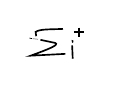
\begin{tikzpicture}[x=.22pt,y=-.22pt,baseline=(sigbase)]
\path[use as bounding box] (0,0) rectangle (110,65);
\coordinate (sigbase) at (0,45);
\node[anchor=base west,inner sep=0,outer sep=0] at (0,45) {\phantom{$\Sigma_i^+$}};
% Complete primary Sigma_i^+; detached head/retrace/independent-rule role unresolved here.
\draw[line width=.6pt] (14,14) -- (13,7) .. controls (20,2) and (37,3) .. (58,2);
\draw[line width=.25pt] (3,17) -- (7,18);
\draw[black!50,line width=.25pt] (8,18) -- (17,19);
\draw[line width=.6pt] (21,20) -- (45,25) .. controls (53,28) and (35,35) .. (5,46) -- (62,43);
\draw[line width=.6pt] (73,29) -- (74,51);
\fill (72,20) -- (75,21) -- (75,24) -- (73,25) -- cycle;
\draw[line width=.65pt] (84,0) -- (84,16);
\draw[line width=.65pt] (76,7) -- (92,7);
\end{tikzpicture}}
% END B024-S01
, % BEGIN B024-S02

\begin{tikzpicture}[x=.22pt,y=-.22pt,baseline=(sigbase)]
\path[use as bounding box] (0,0) rectangle (110,65);
\coordinate (sigbase) at (0,45);
\node[anchor=base west,inner sep=0,outer sep=0] at (0,45) {\phantom{$\Sigma_i^-$}};
% Local upper run remains detached; same primary printed under the first-occurrence rule.
\draw[line width=.55pt] (10,4) -- (39,1);
\draw[line width=.5pt] (4,12) -- (28,18) .. controls (40,22) and (23,36) .. (5,45) .. controls (3,49) and (30,43) .. (40,46) .. controls (46,47) and (45,54) .. (44,58);
\draw[line width=.6pt] (52,30) .. controls (54,33) and (54,37) .. (52,40);
\draw[line width=.6pt] (66,3) -- (87,3);
\end{tikzpicture}
% END B024-S02
les deux comp. \unsure{conn|connexes} de $X\setminus E_i$, alors a) se \unsure{prècise|précise|prêcise} en : il y a \unsure{exactemt|exactement} \uline{un} 
% BEGIN B024-G10
% Complete candidates U_{s_+} | U_{s_-}; no inferred earlier state of the filled sign.
\unsure{\begin{tikzpicture}[x=.18pt,y=-.18pt,baseline=(ubase)]
\path[use as bounding box] (0,0) rectangle (115,120);
\coordinate (ubase) at (0,73);
\node[anchor=base west,inner sep=0,outer sep=0] at (0,73) {\phantom{$U_{s_+}$}};
\draw[line width=.6pt] (2,16) .. controls (8,-3) and (15,1) .. (22,27) .. controls (24,40) and (24,59) .. (29,63) .. controls (34,69) and (48,22) .. (50,7) .. controls (50,37) and (47,64) .. (53,70) .. controls (62,80) and (70,65) .. (78,63);
\draw[line width=.45pt] (78,63) .. controls (83,58) and (87,61) .. (79,67) .. controls (77,70) and (84,82) .. (86,83) -- (90,87) -- (80,90);
\fill (91,96) -- (95,92) -- (104,92) -- (105,89) -- (107,92) -- (115,92) -- (115,97) -- (109,102) -- (113,104) -- (114,108) -- (95,109) -- (91,106) -- cycle;
\node[anchor=base west,inner sep=0,outer sep=0] at (0,73) {\unsure{\begin{tikzpicture}[x=.18pt,y=-.18pt,baseline=(unearbase)]
\path[use as bounding box] (0,0) rectangle (115,120);
\coordinate (unearbase) at (0,73);
\draw[black!35,line width=.6pt] (101,80) -- (103,77);
\fill[black!45] (110,77) circle (.9);
\end{tikzpicture}}};
\end{tikzpicture}}
% END B024-G10
contenu dans 
% BEGIN B024-S03
\unsure{
\begin{tikzpicture}[x=.22pt,y=-.22pt,baseline=(sigbase)]
\path[use as bounding box] (0,0) rectangle (110,65);
\coordinate (sigbase) at (0,45);
\node[anchor=base west,inner sep=0,outer sep=0] at (0,45) {\phantom{$\Sigma_i^{+|-}$}};
% Complete candidates Sigma_i^+ | Sigma_i^-; filled raised sign remains qualified locally.
\draw[line width=.65pt] (3,7) .. controls (25,3) and (36,4) .. (58,4);
\draw[line width=.6pt] (22,7) .. controls (54,18) and (41,19) .. (8,40) .. controls (-2,48) and (35,43) .. (60,46) .. controls (66,48) and (66,55) .. (63,58);
\draw[line width=.65pt] (72,25) .. controls (75,21) and (74,30) .. (72,35);
\fill (82,5) -- (87,5) -- (88,3) -- (90,5) -- (95,5) -- (97,9) -- (97,16) -- (83,16) -- (80,12) -- cycle;
\end{tikzpicture}}
% END B024-S03
tel que $\overline{U_{s_+}}\cap E_i\ne\varnothing$ (et de $=$ pour 
% BEGIN B024-S04
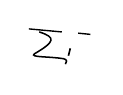
\begin{tikzpicture}[x=.22pt,y=-.22pt,baseline=(sigbase)]
\path[use as bounding box] (0,0) rectangle (110,65);
\coordinate (sigbase) at (0,45);
\node[anchor=base west,inner sep=0,outer sep=0] at (0,45) {\phantom{$\Sigma_i^-$}};
\draw[line width=.5pt] (2,2) -- (56,7);
\draw[line width=.55pt] (19,7) .. controls (47,16) and (45,23) .. (11,43) .. controls (3,49) and (35,47) .. (59,51) .. controls (65,52) and (65,57) .. (62,60);
\draw[line width=.6pt] (70,34) -- (67,46);
\draw[line width=.5pt] (83,9) -- (103,11);
\end{tikzpicture}
% END B024-S04
, \unsure{de|dé|qui} 
% BEGIN B024-G11
% Complete word definit (no accent); the final i body is dotless so its two observed upper pieces are not duplicated.
\begin{tikzpicture}[x=1ex,y=1ex,baseline=(definitword.base)]
\node[anchor=base west,inner sep=0,outer sep=0] (definitword) at (0,0) {defin\i{}t};
\node[anchor=base west,inner sep=0,outer sep=0] at (0,0) {\unsure{\begin{tikzpicture}[x=1ex,y=1ex,baseline=0pt]
\path[use as bounding box] (0,0) rectangle (6.2,2.4);
\draw[black!45,line width=.25pt] (4.95,1.16) -- (4.84,1.66);
\fill (4.78,1.64) circle (.07);
\fill (5.2,1.55) -- (5.25,1.28) -- (5.4,1.24) -- (5.34,1.46) -- cycle;
\end{tikzpicture}}};
\end{tikzpicture}
% END B024-G11
un $U_{s_-}\subset$ 
% BEGIN B024-S05
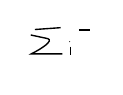
\begin{tikzpicture}[x=.22pt,y=-.22pt,baseline=(sigbase)]
\path[use as bounding box] (0,0) rectangle (110,65);
\coordinate (sigbase) at (0,45);
\node[anchor=base west,inner sep=0,outer sep=0] at (0,45) {\phantom{$\Sigma_i^-$}};
% This complete local form was settled on half b, not reopened for a crop.
\draw[line width=.5pt] (12,3) -- (54,0);
\draw[line width=.5pt] (5,12) -- (33,18) .. controls (43,21) and (24,34) .. (6,43) -- (57,43);
\draw[line width=.5pt] (70,31) -- (70,45);
\fill (69,23) circle (.9);
\draw[line width=.5pt] (84,4) -- (103,4);
\end{tikzpicture}
% END B024-S05
tel que $\overline{U_{s_-}}\cap E_i\ne\varnothing$),
% END B024-P05

% BEGIN B024-ARCHIVE
% archive sheet number: 23
% END B024-ARCHIVE
